\documentclass[fontsize=11pt]{scrartcl}
%-------------------------------------------------------------------------------------------------
% LATEX TEMPLATE FOR A BACHELOR'S THESIS AT GHENT UNIVERSITY GLOBAL CAMPUS
% CREATED BY MANVEL GASPARYAN
% APRIL, 2021
%-------------------------------------------------------------------------------------------------
\usepackage{hyperref, tikz, float, subfigure, multicol, amsmath, amsthm, alphalph, amsfonts, amssymb, geometry, enumitem, parskip, xcolor, sectsty}
\usepackage[normalem]{ulem}
\usepackage[font=scriptsize,labelfont=bf]{caption}
\usepackage[explicit]{titlesec}
\usepackage[scaled]{helvet}
\renewcommand\familydefault{\sfdefault} 
\usepackage[T1]{fontenc}

\usepackage{setspace}

\usepackage{{listings}}

\usepackage{graphicx}
\usepackage{float} 
\usepackage{subfigure}

%-------------------------------------------------------------------------------------------------
 \geometry{a4paper, total={170mm,257mm}, left=20mm, right=20mm, top=25mm, bottom=30mm}
%-------------------------------------------------------------------------------------------------
\newtheorem{proposition}{Proposition}[section]
\newtheorem{lemma}{Lemma}[section]
\newtheorem{remark}{Remark}[section]
\newtheorem{corollary}{Corollary}[section]
\newtheorem{definition}{Definition}[section]
%-------------------------------------------------------------------------------------------------
\pagenumbering{roman}
\usepackage{fancyhdr}
\pagestyle{fancy}
\fancyhf{}
\renewcommand{\headrulewidth}{0pt}
\rhead{}
\lhead{}
\rfoot{\thepage}
\lfoot{}

%-------------------------------------------------------------------------------------------------
\definecolor{ghent_blue}{rgb}{0.1176, 0.392, 0.7843}
\definecolor{ghent_dark}{rgb}{0.0, 0.2, 0.4}
%-------------------------------------------------------------------------------------------------
\title{{\color{ghent_blue} TITLE: LATEX TEMPLATE FOR A BACHELOR'S THESIS AT GHENT UNIVERSITY GLOBAL CAMPUS}}
\subtitle{{\color{ghent_dark} [DOCUMENT SUBTITLE]}}
\date{}         
%-------------------------------------------------------------------------------------------------
\sectionfont{\fontsize{16}{15}\selectfont}
\sectionfont{\color{ghent_blue}}
%=================================================================================================
\begin{document}
%=================================================================================================
%PAGE i: TITLE PAGE 1
%-------------------------------------------------------------------------------------------------
\thispagestyle{empty}
\hfill
\includegraphics[scale = 1]{img/badge/2021.png}\\
%-------------------------------------------------------------------------------------------------
\vspace{8cm}

\noindent{\fontsize{30}{50}\selectfont{\color{ghent_blue}\noindent \hspace{12mm}\textbf{
Microphotonics %TITLE
}}}\\
\fontsize{20}{50}\selectfont{\color{ghent_dark}\noindent \hspace{13mm}\textbf{
CAD-LAB: Fourier Optics%SUBTITLE
}}\vspace{10mm}

\hspace{10mm}{\fontsize{10}{10}\selectfont{\textbf{
Lukuan Zhang, Rui Zhu, Xiyuan Guo%AUTHOR
}}}
\vspace*{\fill}
%-------------------------------------------------------------------------------------------------
\begin{flushleft}
\begin{figure}[b!]

\includegraphics[scale = 1.4]{img/badge/GUGC.pdf}
\end{figure}
\end{flushleft}

\doublespacing
\tableofcontents
\pagebreak
\pagenumbering{arabic}
%=================================================================================================
%HELP
%-------------------------------------------------------------------------------------------------
\section*{*  \uline{HELP}}
Once have been refered you can delete this part.\\
If you want to write an inline equation, code like this $E=mc^2$.\\
If you want to write a displayed equation without numbering, code like this $$E=mc^2$$\\
If you want to write a numbering displayed equation, code like this
\begin{equation} 
    E=mc^2 \label{eq1}
\end{equation}
and you can quote the equation by using Eq.\ref {eq1}.\\
\textbf{Tips:} The software \verb|Mathpix| can convert images and PDFs to LaTeX format which is
highly recommended by me.\\
List items like this:
\begin{enumerate} % itemize/description
    \item contents
    \item contents
\end{enumerate}
If you want to add one or more images as Figure \ref{name1} shown, you can copy the
code as following.\\
\begin{figure}[H]
    \centering
     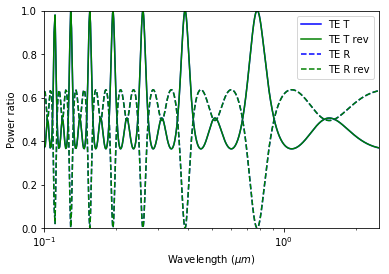
\includegraphics[width=0.35\textwidth]{img/1.png} % set width to get a proper ratio
     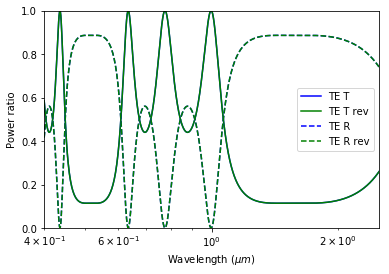
\includegraphics[width=0.35\textwidth]{img/2.png}
     \caption{Here to write the caption of the figure.}
     \label{name1}
\end{figure}
{\color{ghent_blue}Some details to notice:}
\begin{enumerate}
    \item  \textbf{Function name} and \textbf{units} should be presented in the Roman Regular Font.
    We can do this by using the sign backslash such as $\log(x)$, $\sin(x)$, $\cos(x)$, etc.
    \item When writing source codes in \LaTeX, make sure that the one-line code length 
    \textbf{does not} exceed one page(or 1/2 screen width on computer). Too long in width makes 
    a worse reading experience.
    \item Everytime when the new task comes, you are allowed to copy the whole template file and 
    rename it into the task name, then modify on the copy. Please don't modify the code directly
    on the template.
    \item Don't forget enter a space after the punstuation marks.
\end{enumerate}



%=================================================================================================
\pagebreak
%=================================================================================================
%TASK 1
%-------------------------------------------------------------------------------------------------
\section{\uline{TASK 1}}
%-------------------------------------------------------------------------------------------------
Suppose that the circle aperture lies in the $(x', y')$ plane and 
the observed point lies in the $(x, y)$ plane. The distance between 
$(x', y')$ and $(x, y)$ can be written as binominal series:
\begin{equation}
    \begin{aligned}
    R &=\sqrt{\left(x-x^{\prime}\right)^{2}+\left(y-y^{\prime}\right)^{2}+z^{2}}=\sqrt{\rho^{2}+z^{2}} \\
    &=z \sqrt{1+\frac{\rho^{2}}{z^{2}}} \\
    &=z\left[1+\frac{\rho^{2}}{2 z^{2}}-\frac{1}{8}\left(\frac{\rho^{2}}{z^{2}}\right)^{2}+\cdots\right] \\
    &=z+\frac{\rho^{2}}{2 z}-\frac{\rho^{4}}{8 z^{3}}+\cdots
    \end{aligned}
\end{equation}
with $\rho=\sqrt{\left(x-x^{\prime}\right)^{2}+\left(y-y^{\prime}\right)^{2}}$.

Fresnel approximation is to assum that the third term of the series 
is small enough to ignore, which means
\begin{equation}
    \frac{k \rho^{4}}{8 z^{3}} \ll 2 \pi \Rightarrow 
    z \gg\left(\frac{\rho^{4}}{8 \lambda}\right)^{1 / 3}
    \label{eq2}
\end{equation}
Meanwhile the second term cannot be ignored:
\begin{equation}
    \frac{k \rho^{2}}{2 z^{2}} > 2 \pi \Rightarrow 
    z < \frac{\rho^2}{2\lambda} 
    \label{eq3}
\end{equation}
Fraunhofer approximation assums that the second term is small enough 
as
\begin{equation}
    \frac{k \rho^{2}}{2 z^{2}} \ll 2 \pi \Rightarrow 
    z\gg \frac{\rho^2}{2\lambda} 
    \label{eq4}
\end{equation}
Assum diameter of the observed plane and the circle apperture are the same. 
Put $\lambda = 1.55 \times 10^{-6}m$, $r = \frac{\rho}{2} = 1.5 \times 10^{-4}m$ into
equations above, we get $z$ distance condition of Fresnel diffraction 
$8.68 \times 10^{-4}m \ll z < 2.90 \times 10^{-2}m $
and of Fraunhofer diffraction $z \gg 2.90 \times 10^{-2}m$.


%-------------------------------------------------------------------------------------------------
\subsection{}
%-------------------------------------------------------------------------------------------------
As Fig\ref{fig1.1} shown, with $z$ becoming larger, the intensity of first level circle 
takes more advantage than other level circles. And when $z > 0.029m$, the diffraction shape
matches inferrence, which is consistent with calcuation. 
\begin{figure}[H]
    \centering
     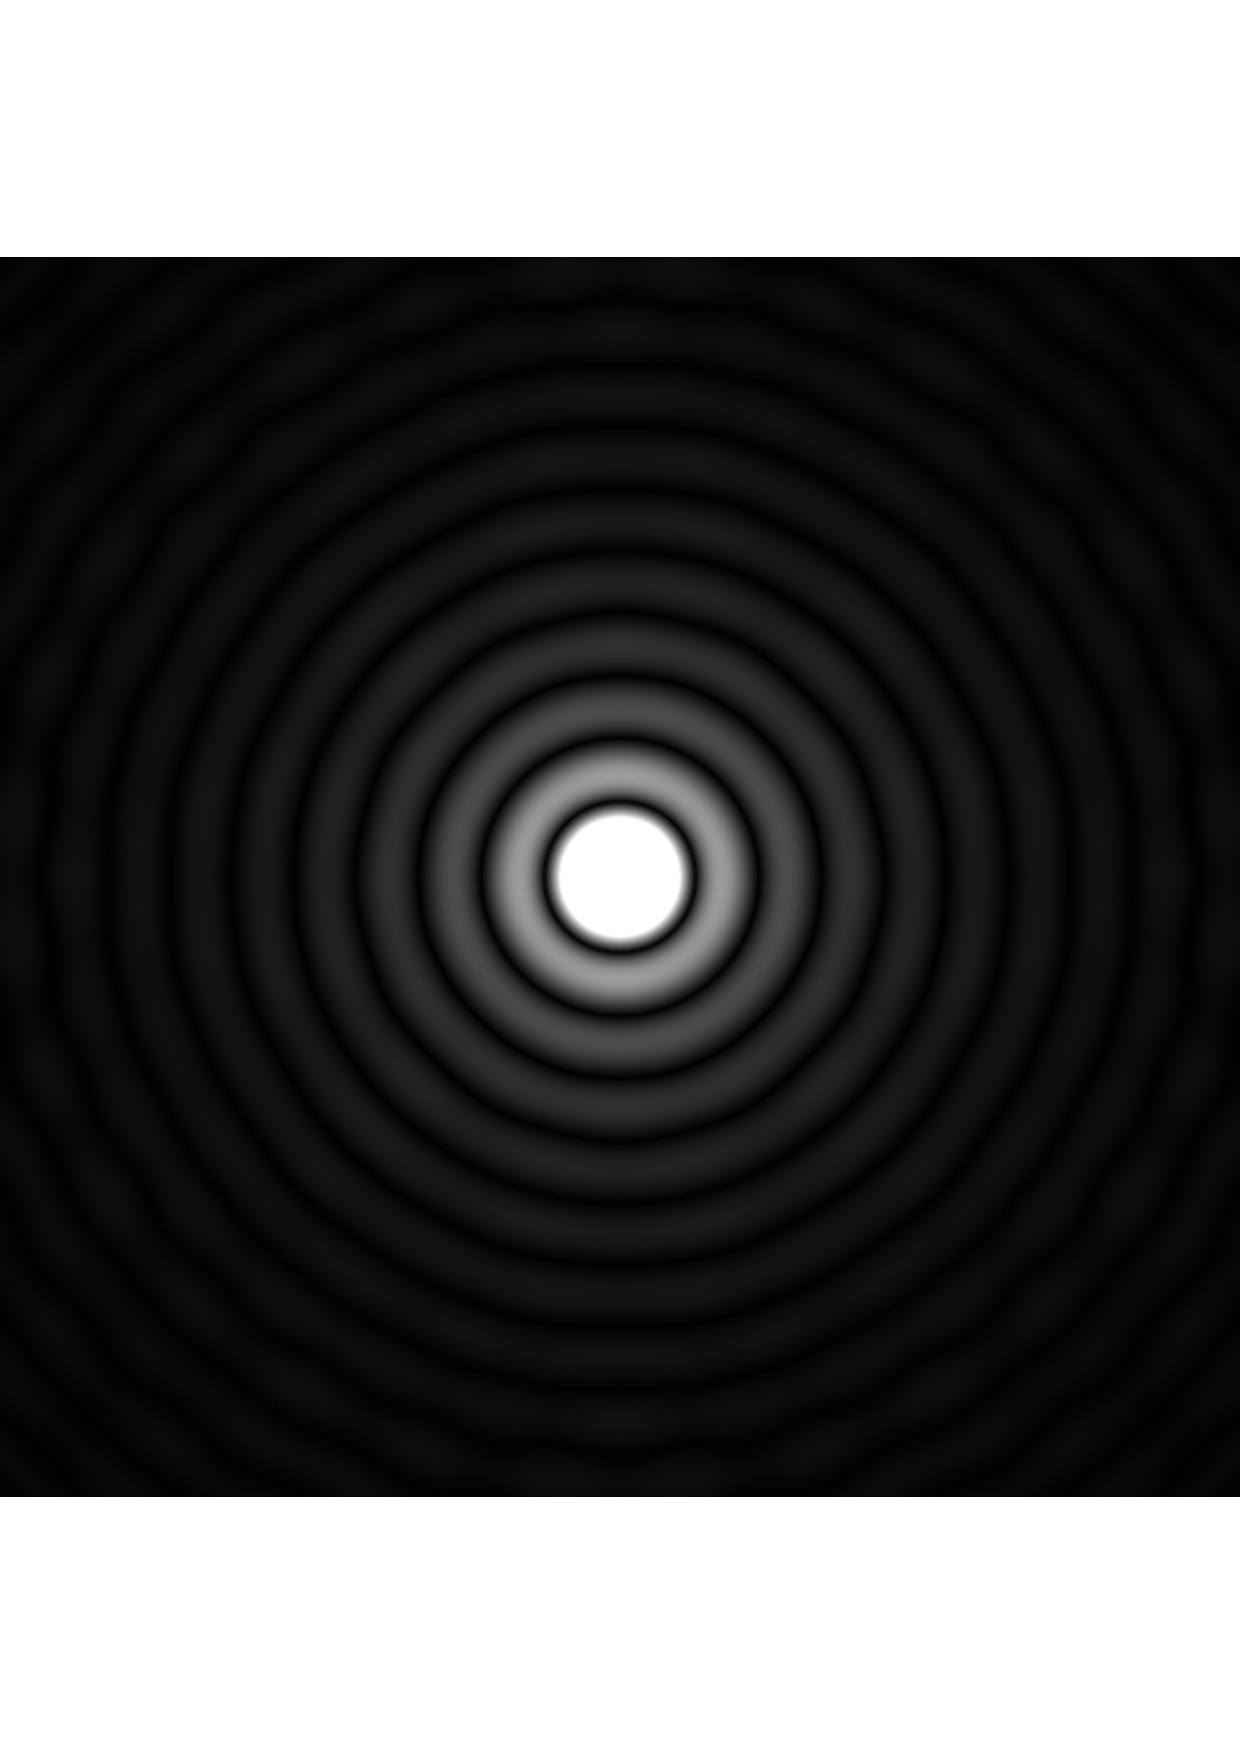
\includegraphics[width=0.20\textwidth]{img/1_Fra_0.01.bmp.pdf}
     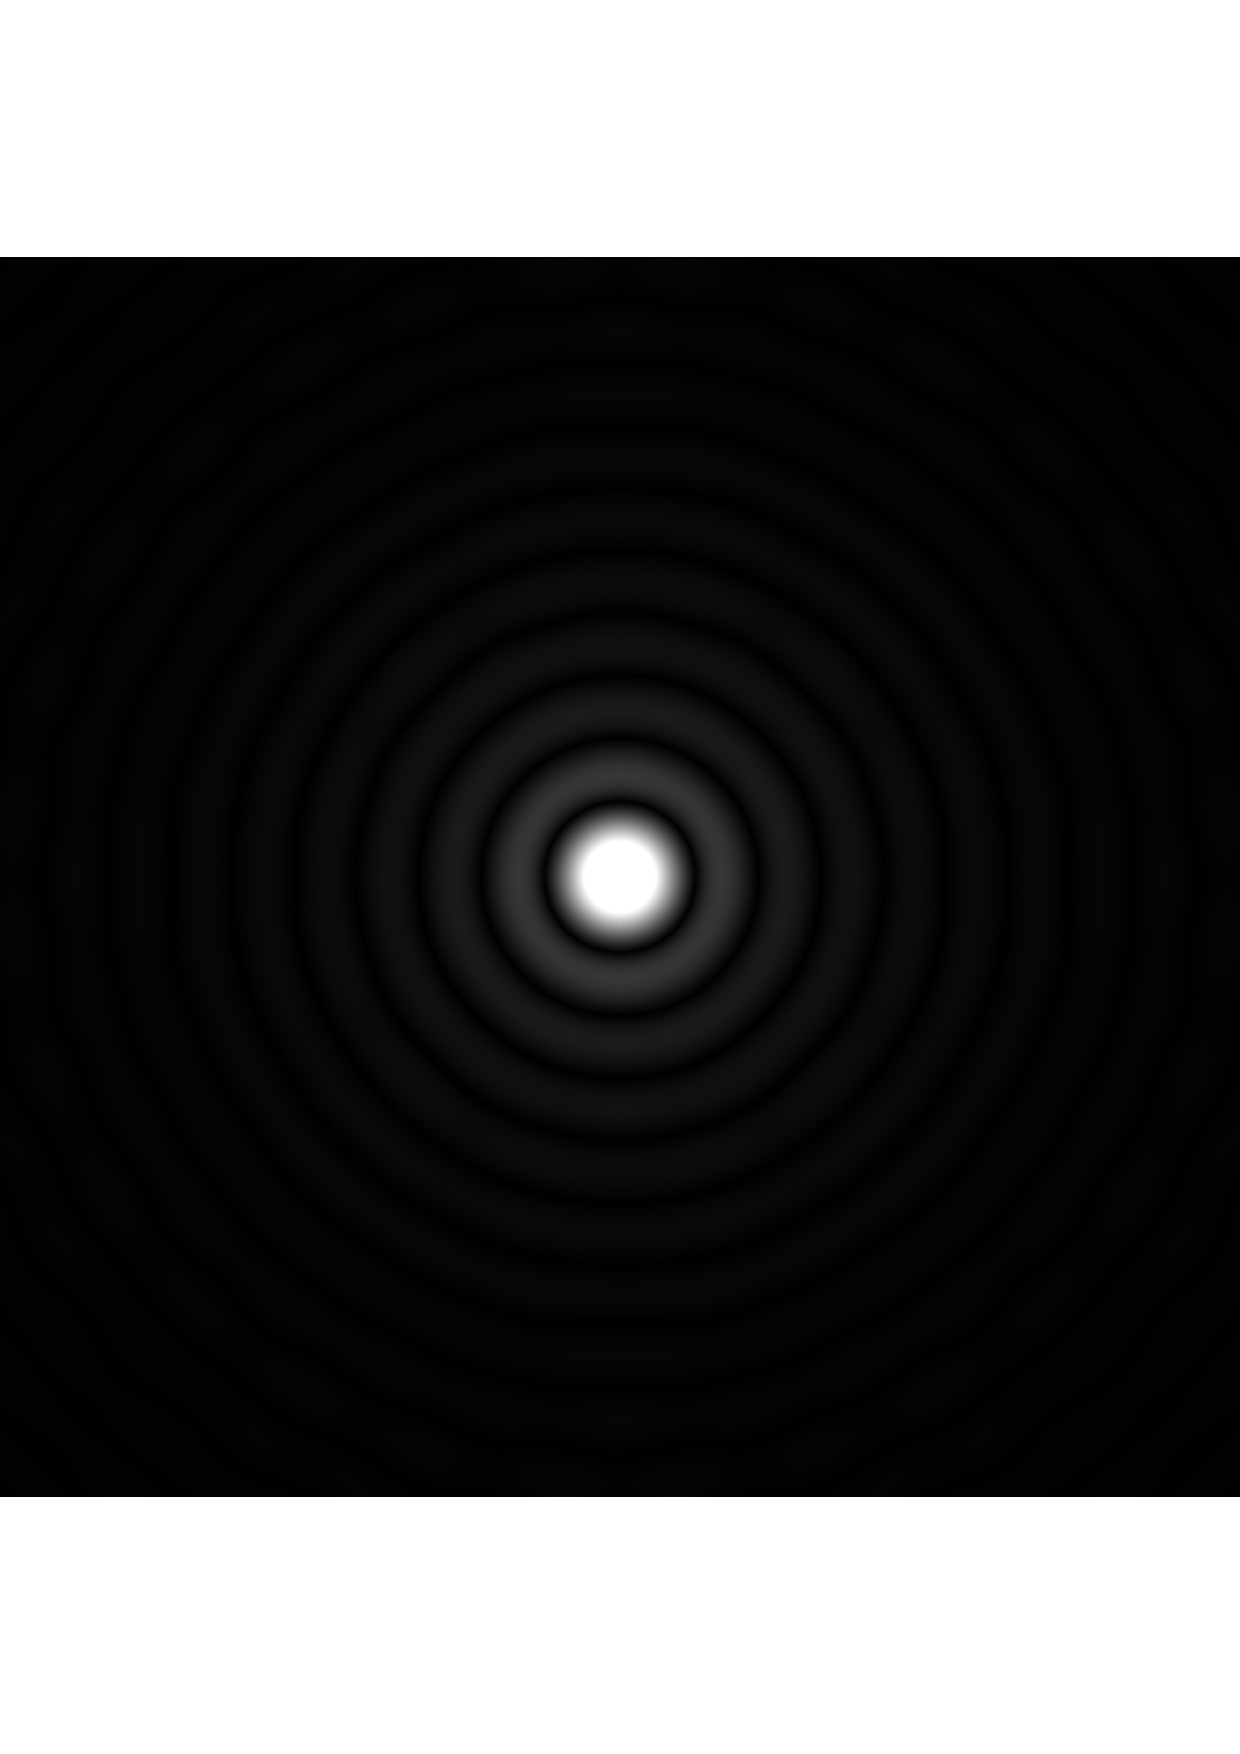
\includegraphics[width=0.20\textwidth]{img/1_Fra_0.029.bmp.pdf}
     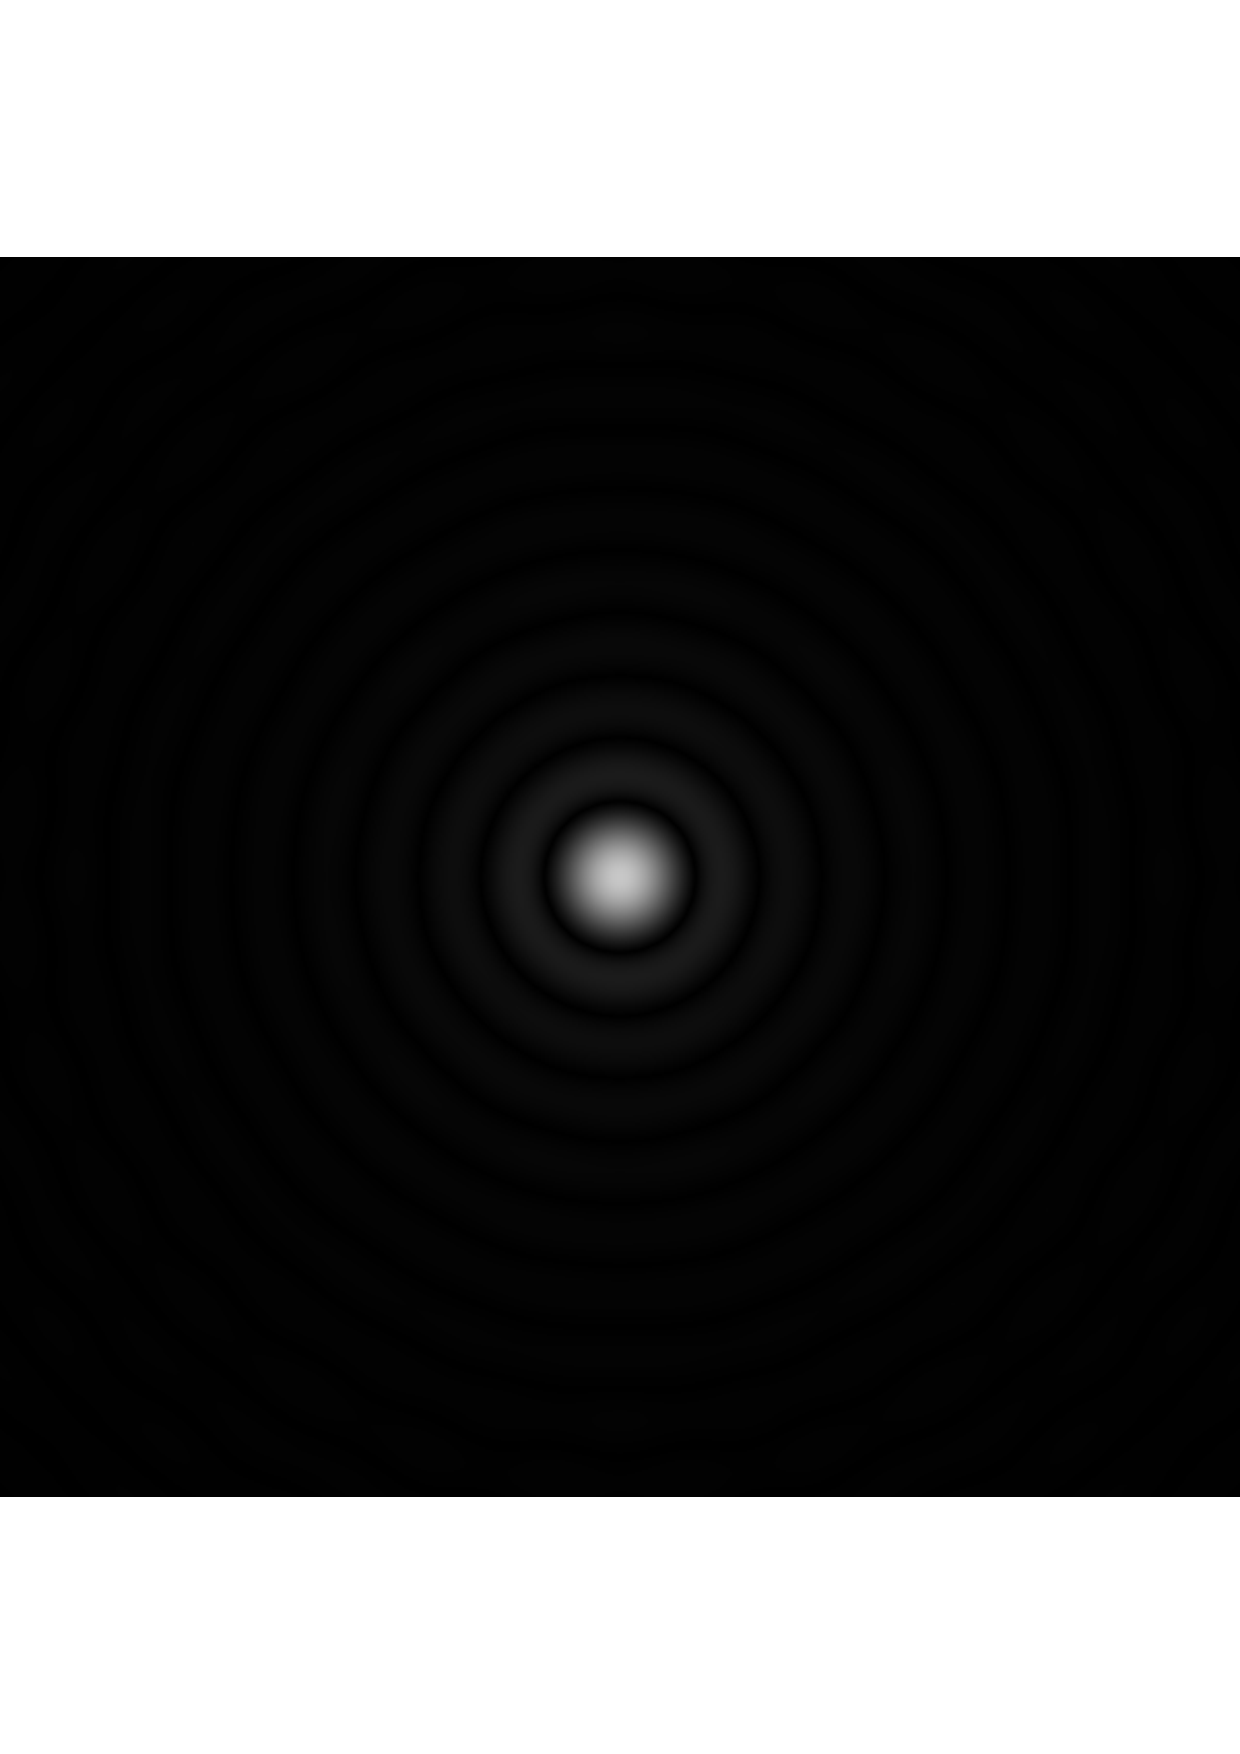
\includegraphics[width=0.20\textwidth]{img/1_Fra_0.058.bmp.pdf}
     
\includegraphics[width=0.20\textwidth]{img/1_Fra_0.116.bmp.pdf}
     \caption{Fraunhofer diffraction when $z = 0.01m, 0.029m, 0.058m$ and $0.116m$.}
     \label{fig1.1}
\end{figure}

%-------------------------------------------------------------------------------------------------
\subsection{}
%-------------------------------------------------------------------------------------------------
According to the calculation, Fresnel approximation is valid when 
$8.68 \times 10^{-4}m \ll z < 2.90 \times 10^{-2}m $. So we take 
$z = 0.0001m, 0.001m, 0.01m$ and $0.1m$ to simulate in both Fresnel diffraction
and Fraunhofer diffraction.
\begin{figure}[H]
    \centering
     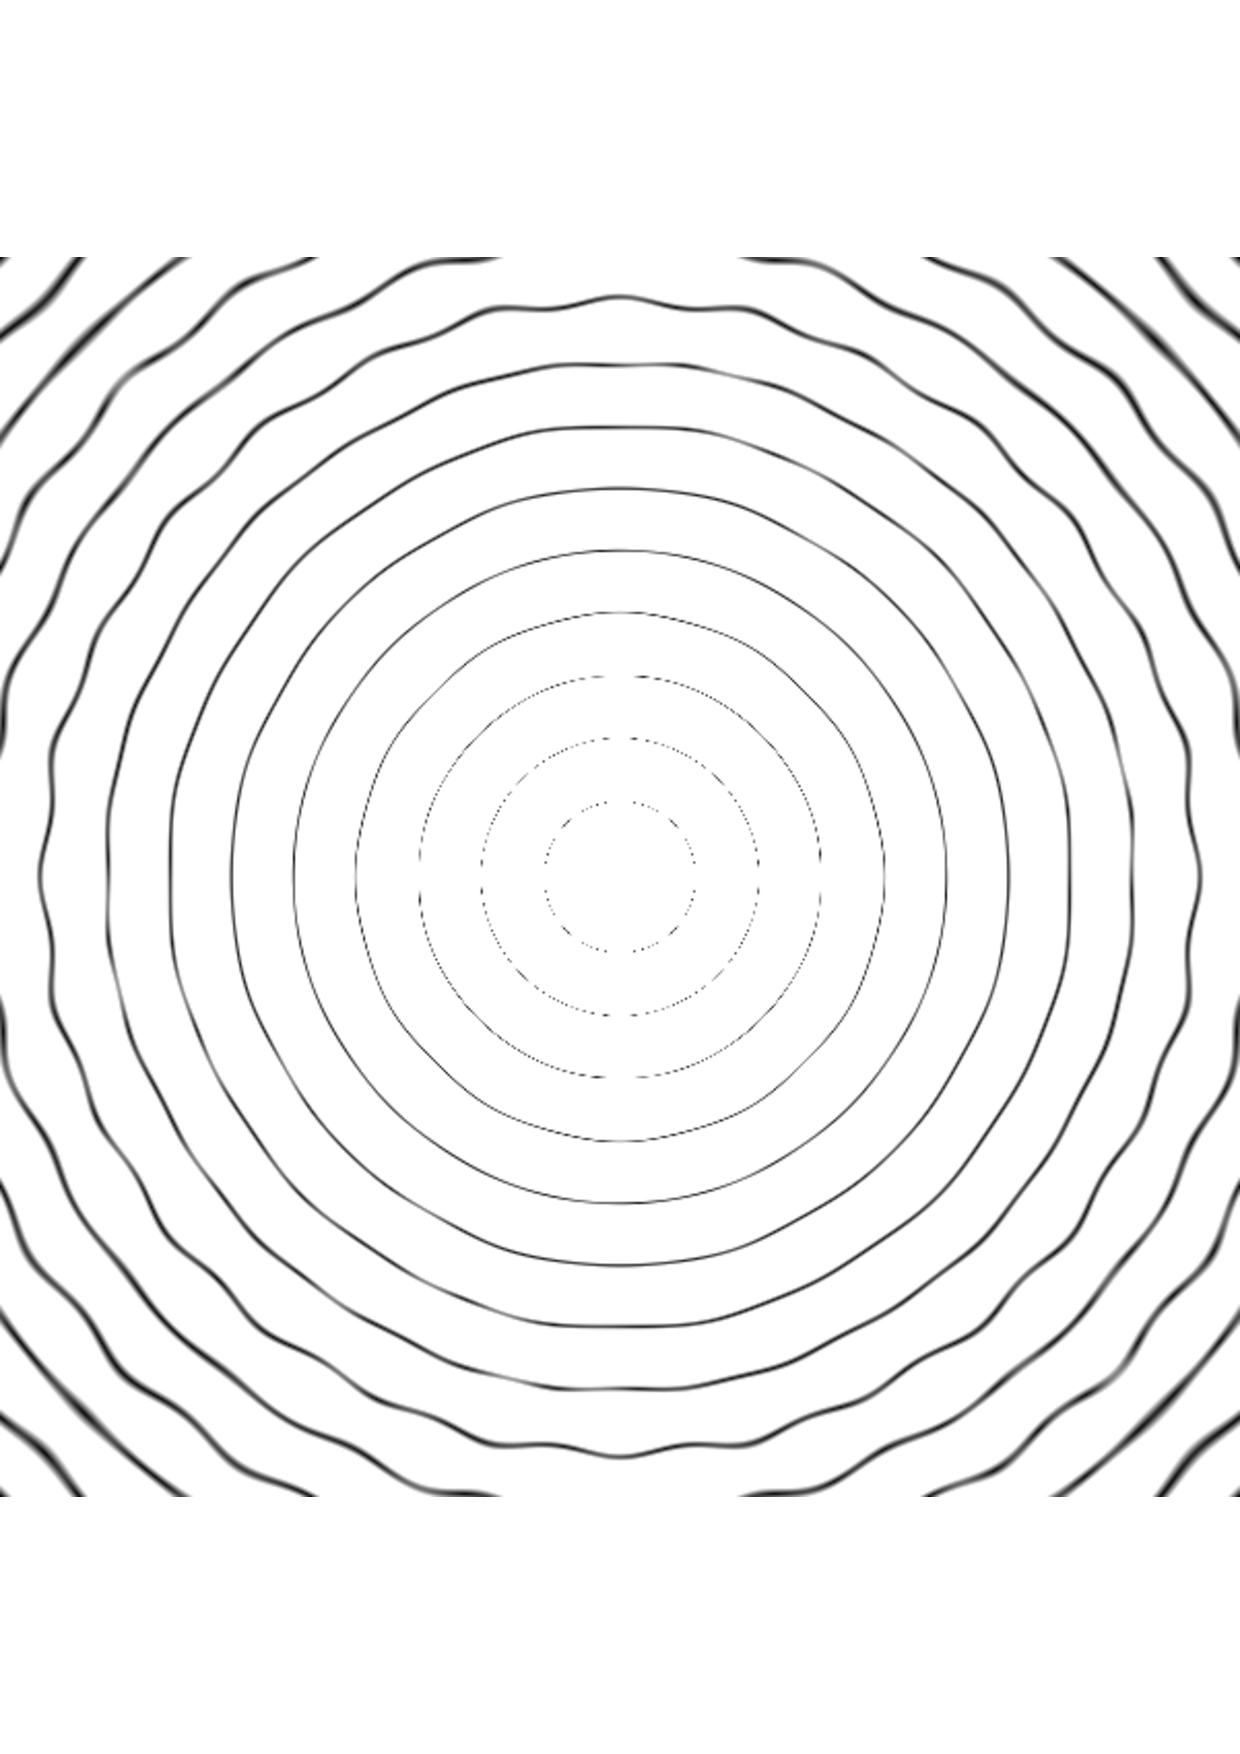
\includegraphics[width=0.20\textwidth]{img/1_Fra_-4.bmp.pdf}
     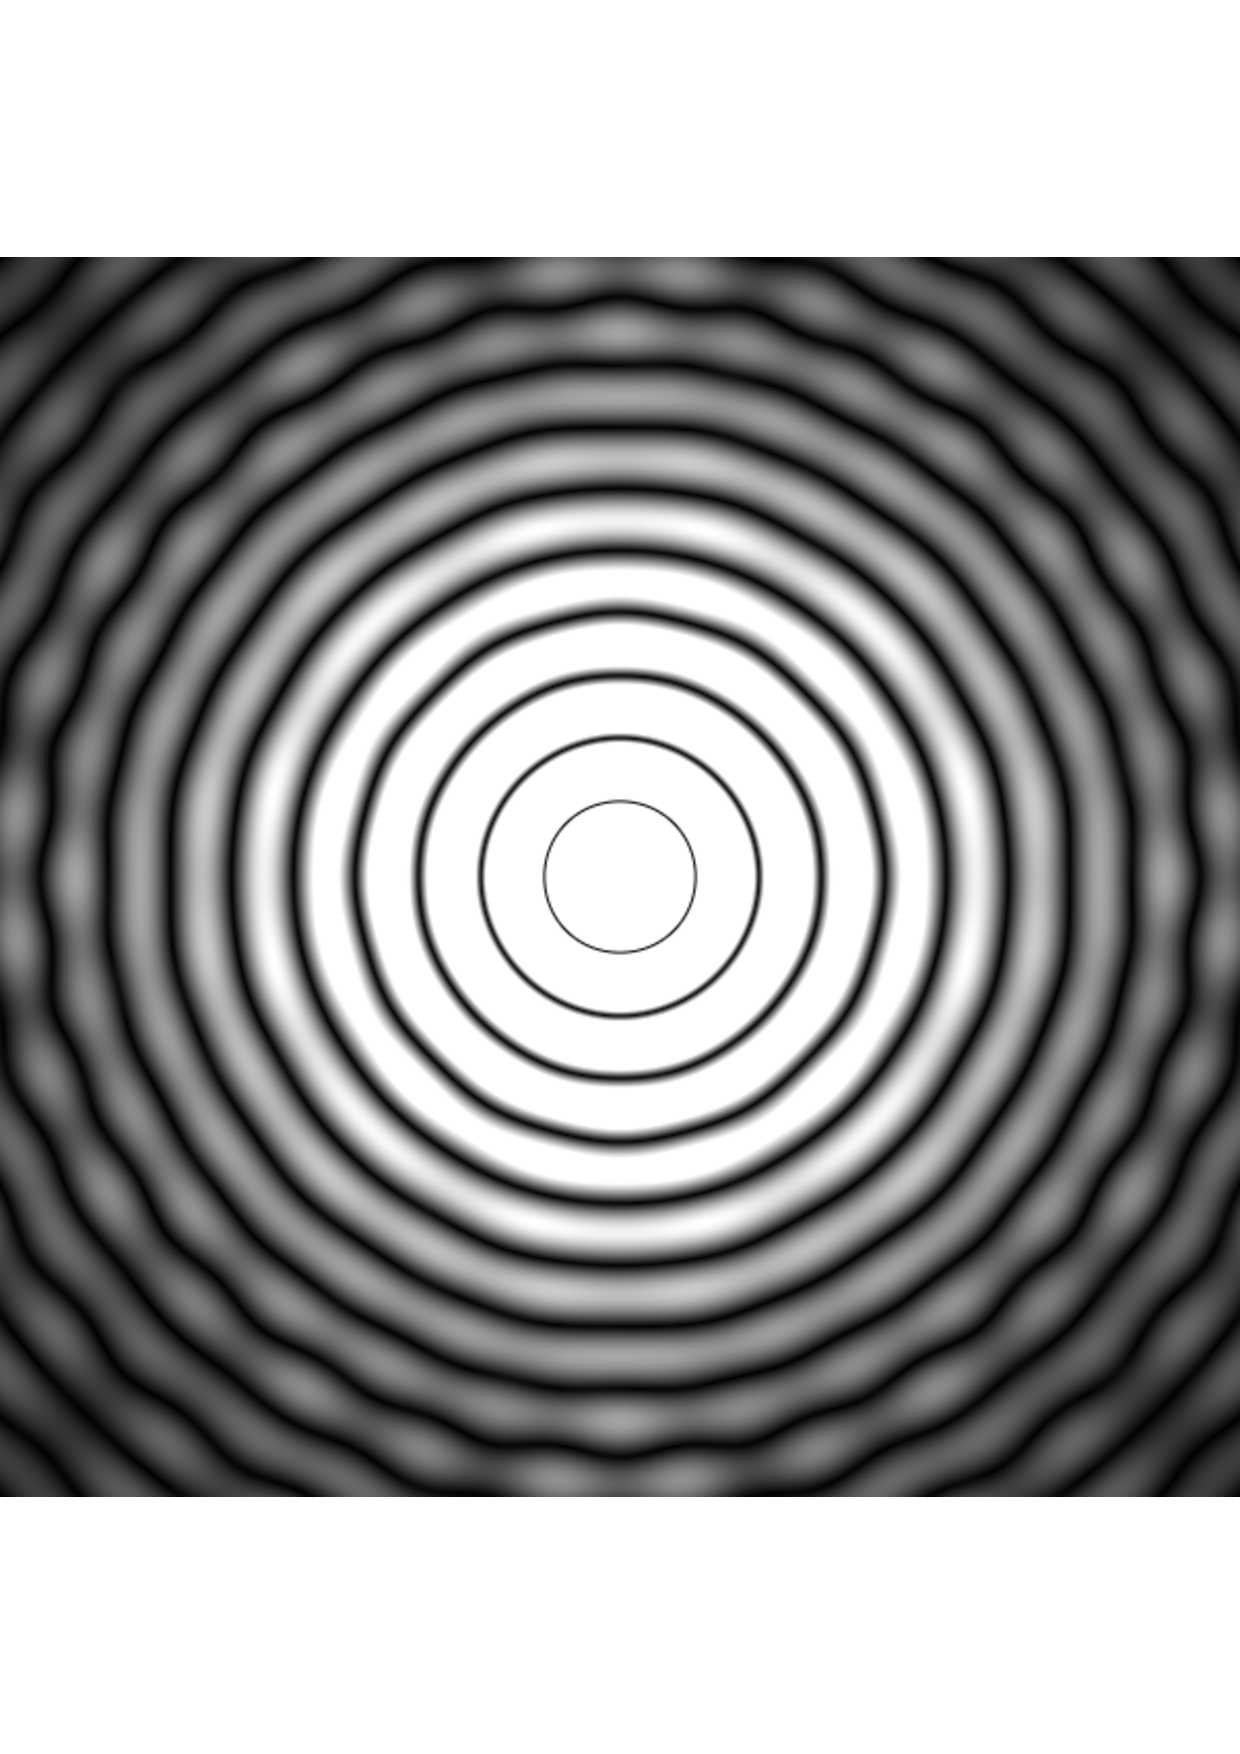
\includegraphics[width=0.20\textwidth]{img/1_Fra_-3.bmp.pdf}
     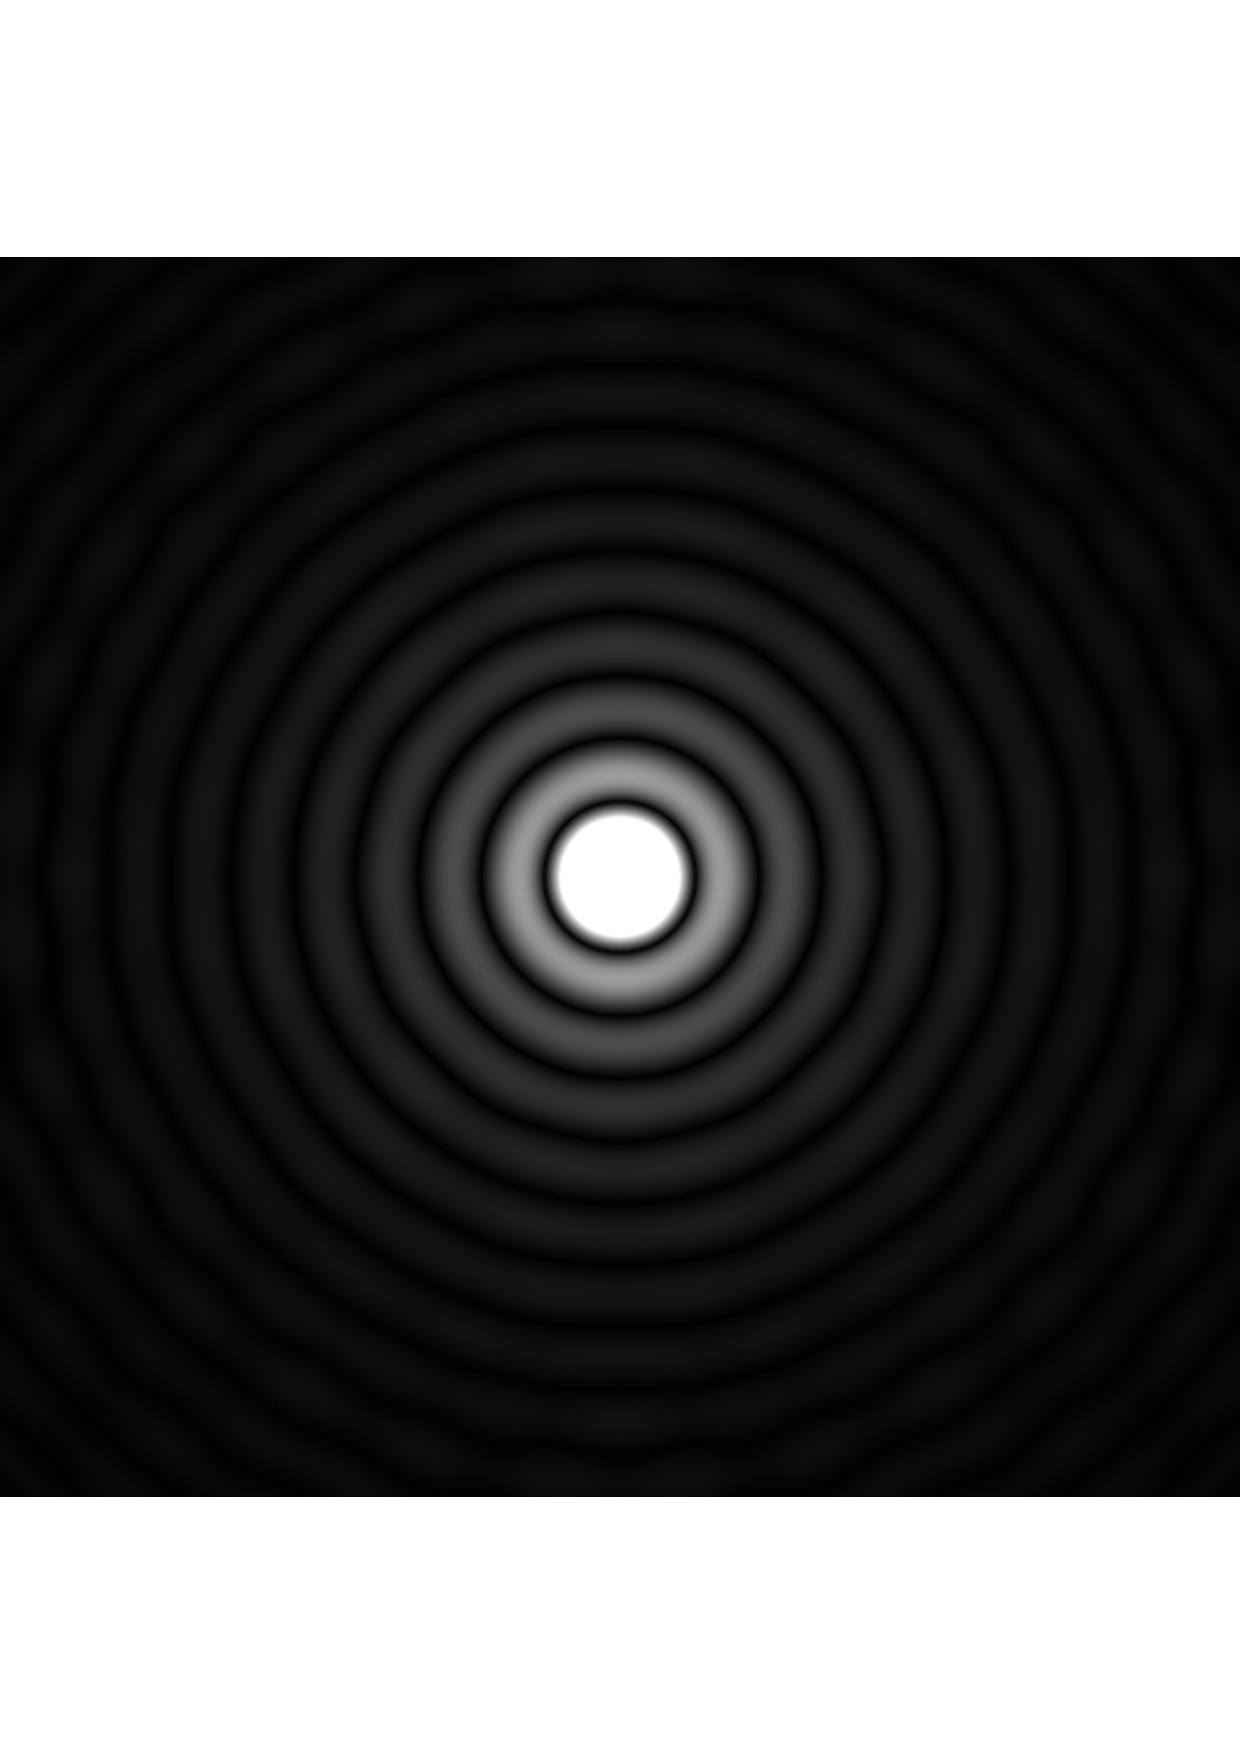
\includegraphics[width=0.20\textwidth]{img/1_Fra_-2.bmp.pdf}
     
\includegraphics[width=0.20\textwidth]{img/1_Fra_-1.bmp.pdf}
     \caption{Fraunhofer diffraction when $z = 0.0001m, 0.001m, 0.01m$ and $0.1m$.}
     \label{fig1.2}
\end{figure}
\begin{figure}[H]
    \centering
     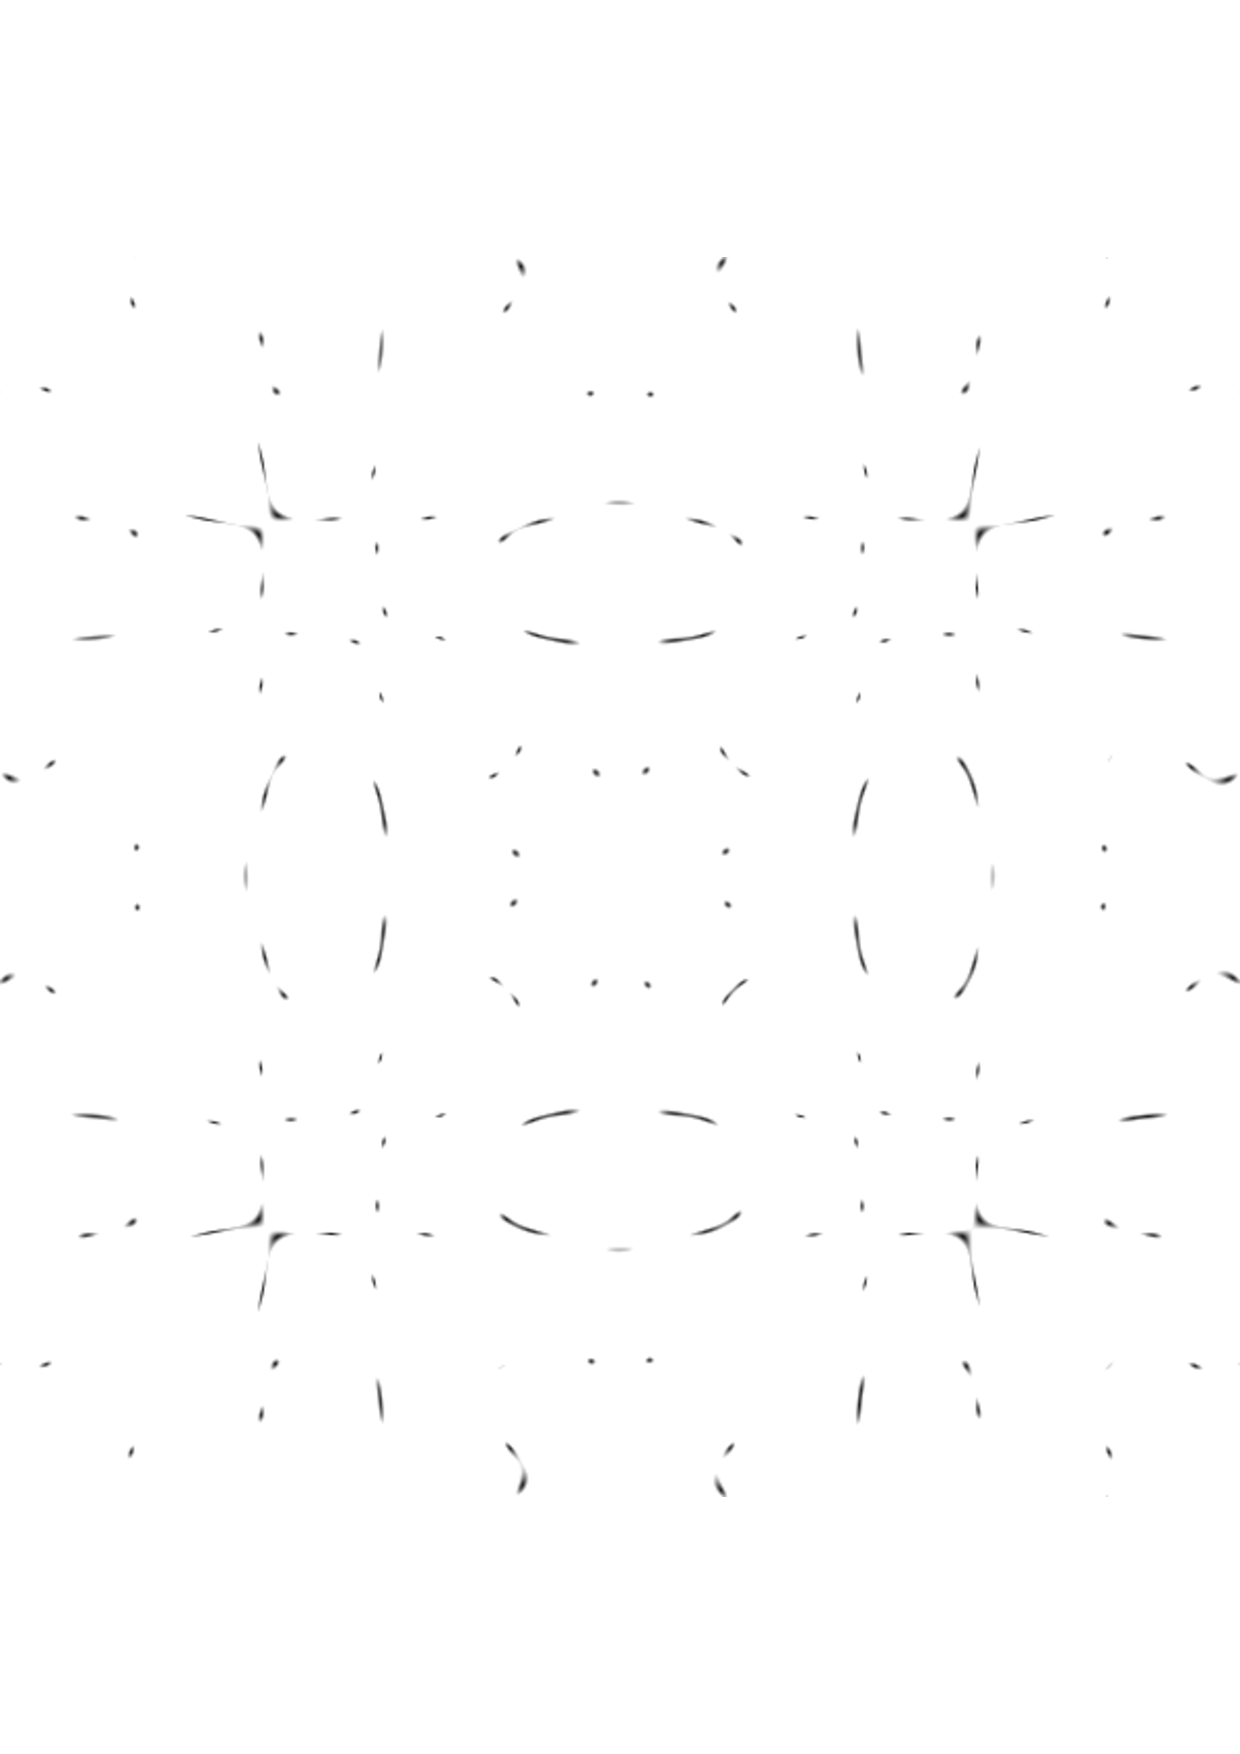
\includegraphics[width=0.20\textwidth]{img/1_Fre_-4.bmp.pdf}
     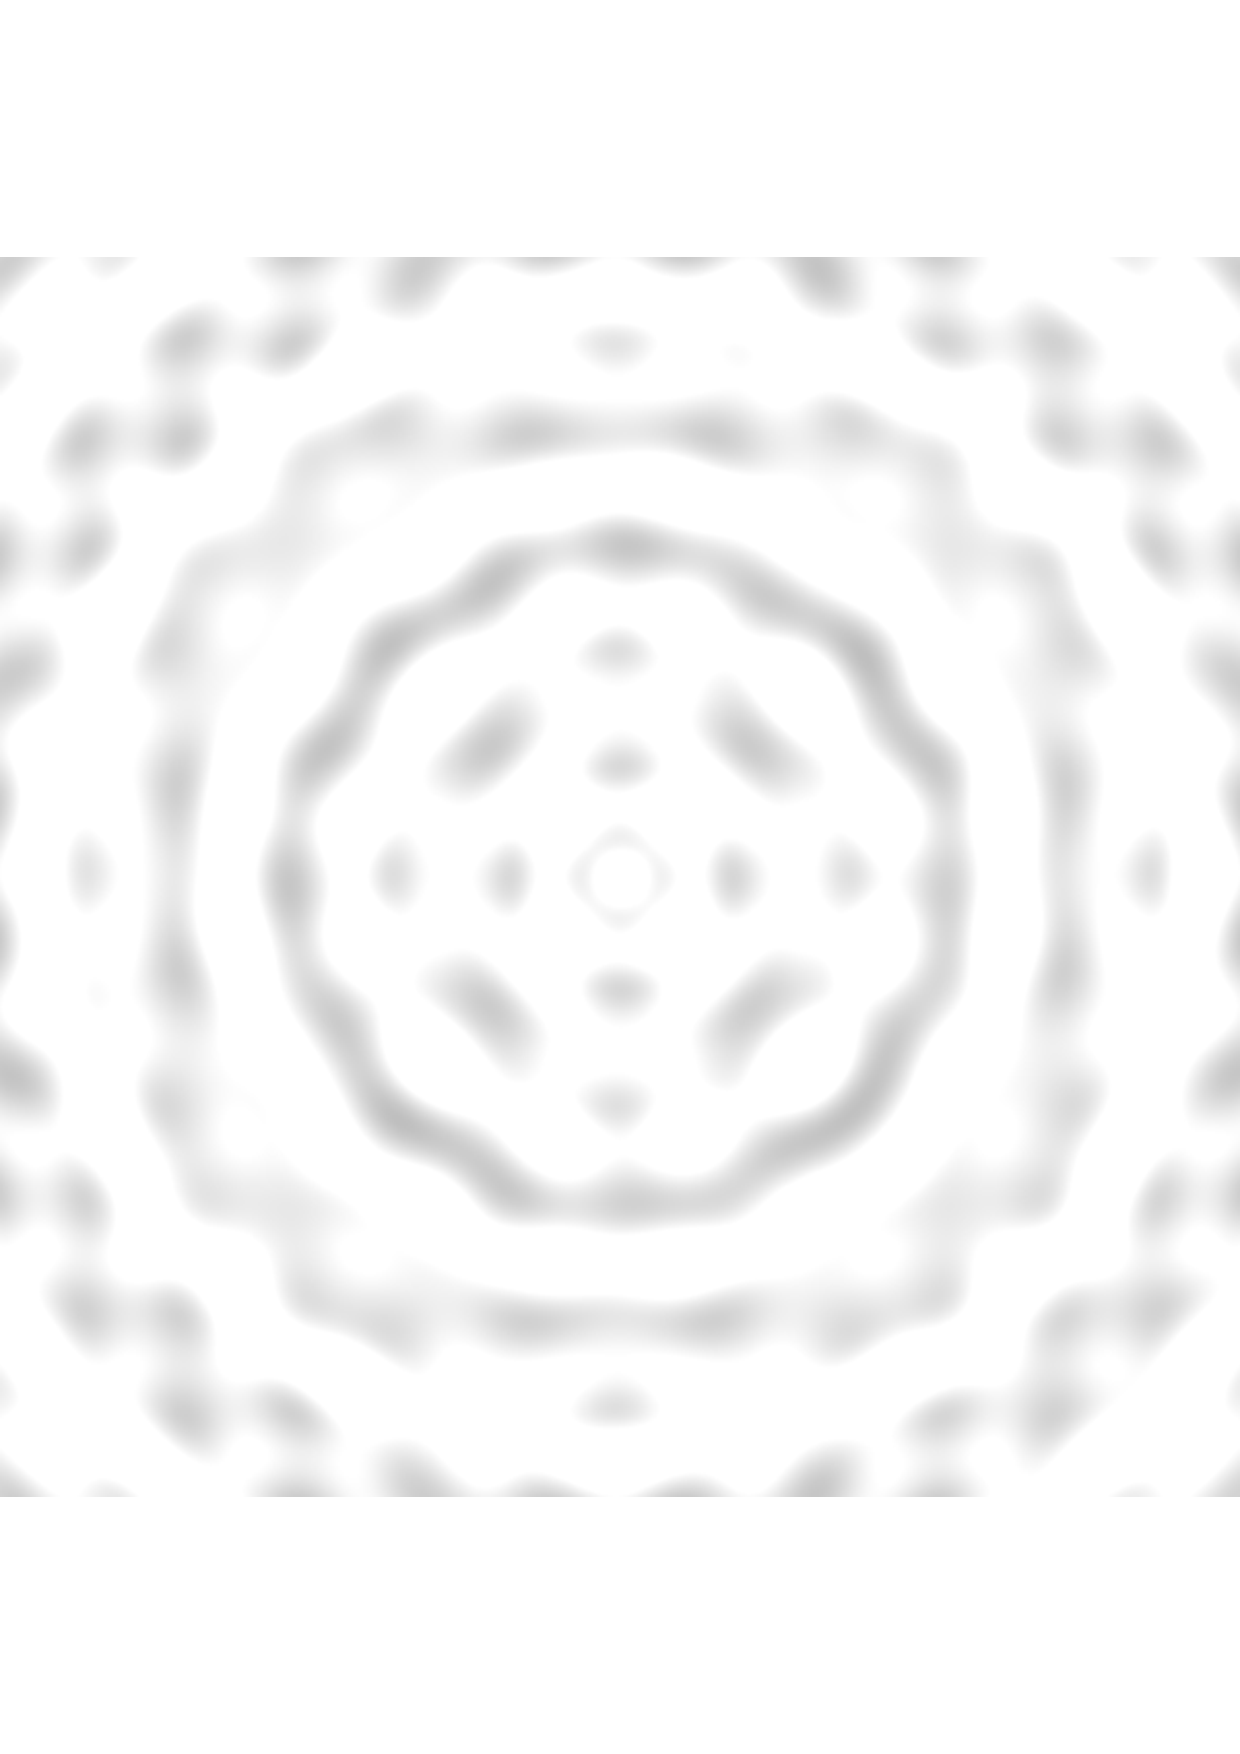
\includegraphics[width=0.20\textwidth]{img/1_Fre_-3.bmp.pdf}
     
\includegraphics[width=0.20\textwidth]{img/1_Fre_-2.bmp.pdf}
     
\includegraphics[width=0.20\textwidth]{img/1_Fre_-1.bmp.pdf}
     \caption{Fresnel diffraction when $z = 0.0001m, 0.001m, 0.01m$ and $0.1m$.}
     \label{fig1.3}
\end{figure}
From \ref{fig1.2}, we can see that Fraunhofer diffraction shapes  
behave similarly, with several circles surrounding the center and darkening
from the inside out. However, with $z$ decreases near to the threshold of 
$8.68 \times 10^{-4}m$, Fresnel diffraction
shapes distort and finally become unrecognizable, consistent with the calculation.
%-------------------------------------------------------------------------------------------------
\subsection{}
%-------------------------------------------------------------------------------------------------
In theory, the position of amplitude zero's goes as
\begin{equation}
    r_0 = \frac{1.22 \lambda z}{2r}
\end{equation}
When $z = 1m$, we get $r_0 = 0.0063m$, correspondent with Fig\ref{fig1.4}
\begin{figure}[H]
    \centering
     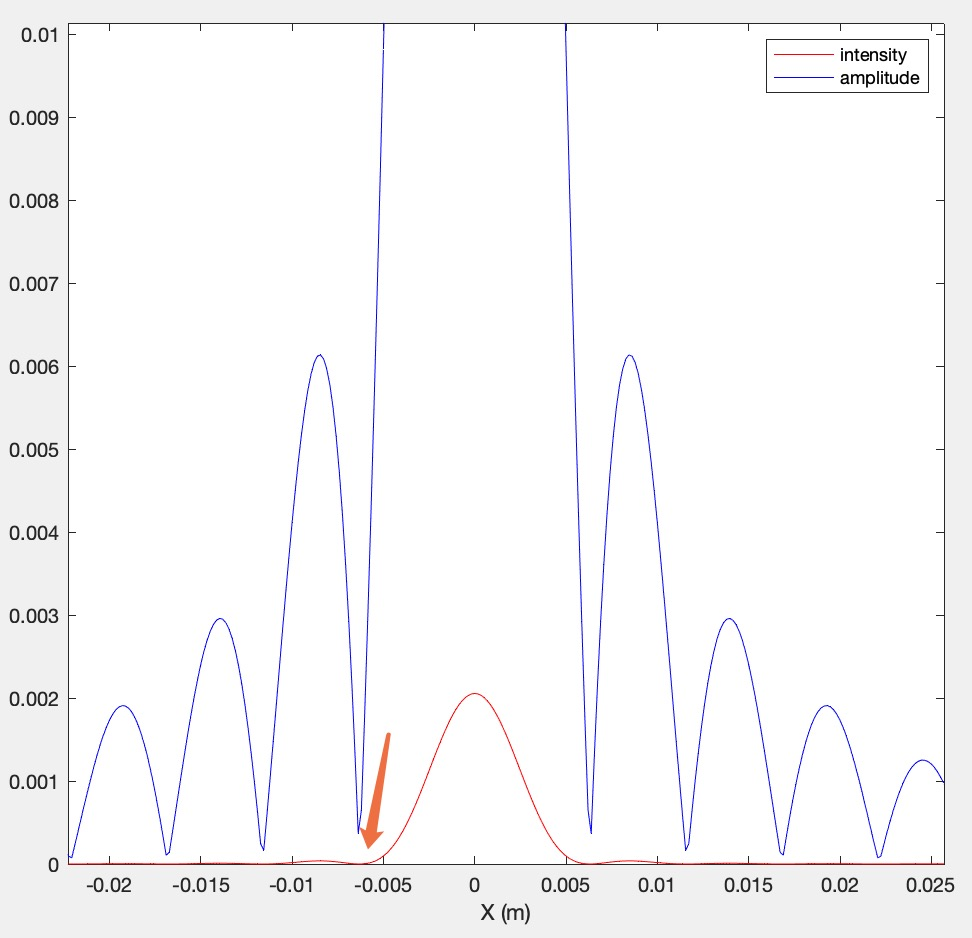
\includegraphics[width=0.50\textwidth]{img/1_3.png}
     \caption{Airy pattern when $z = 1m$.}
     \label{fig1.4}
\end{figure}
%=================================================================================================
\pagebreak
%=================================================================================================
%TASK 2
%-------------------------------------------------------------------------------------------------
\section{\uline{TASK 2}}
%-------------------------------------------------------------------------------------------------
Let $z = 0.05m$. (Being too far will cause a sharp decrease in intenstity, 
unsuitable for observation)

Keep width unchange as $0.0001m$, and change height in
$0.0001m, 0.0005m, 0.001m$ and $0.005m$. The diffraction patterns
are shown as below. When height increases, the diffraction stripes
in the perpendicular direction become longer and brighter. If height
tends to infinity, the diffraction pattern will transform to the 
slit diffraction. We can see it from
\begin{equation}
    I\left(x_{0}, y_{0}\right)=\left(\frac{\ell_{x} \ell_{y}}{\lambda z}\right)^{2} \operatorname{sinc}^{2}\left(\frac{\pi \ell_{x} x_{0}}{\lambda z}\right) \operatorname{sinc}^{2}\left(\frac{\pi \ell_{y} y_{0}}{\lambda z}\right)
\end{equation}

\begin{figure}[H]
    \centering
     
\includegraphics[width=0.20\textwidth]{img/2_0.bmp.pdf}
     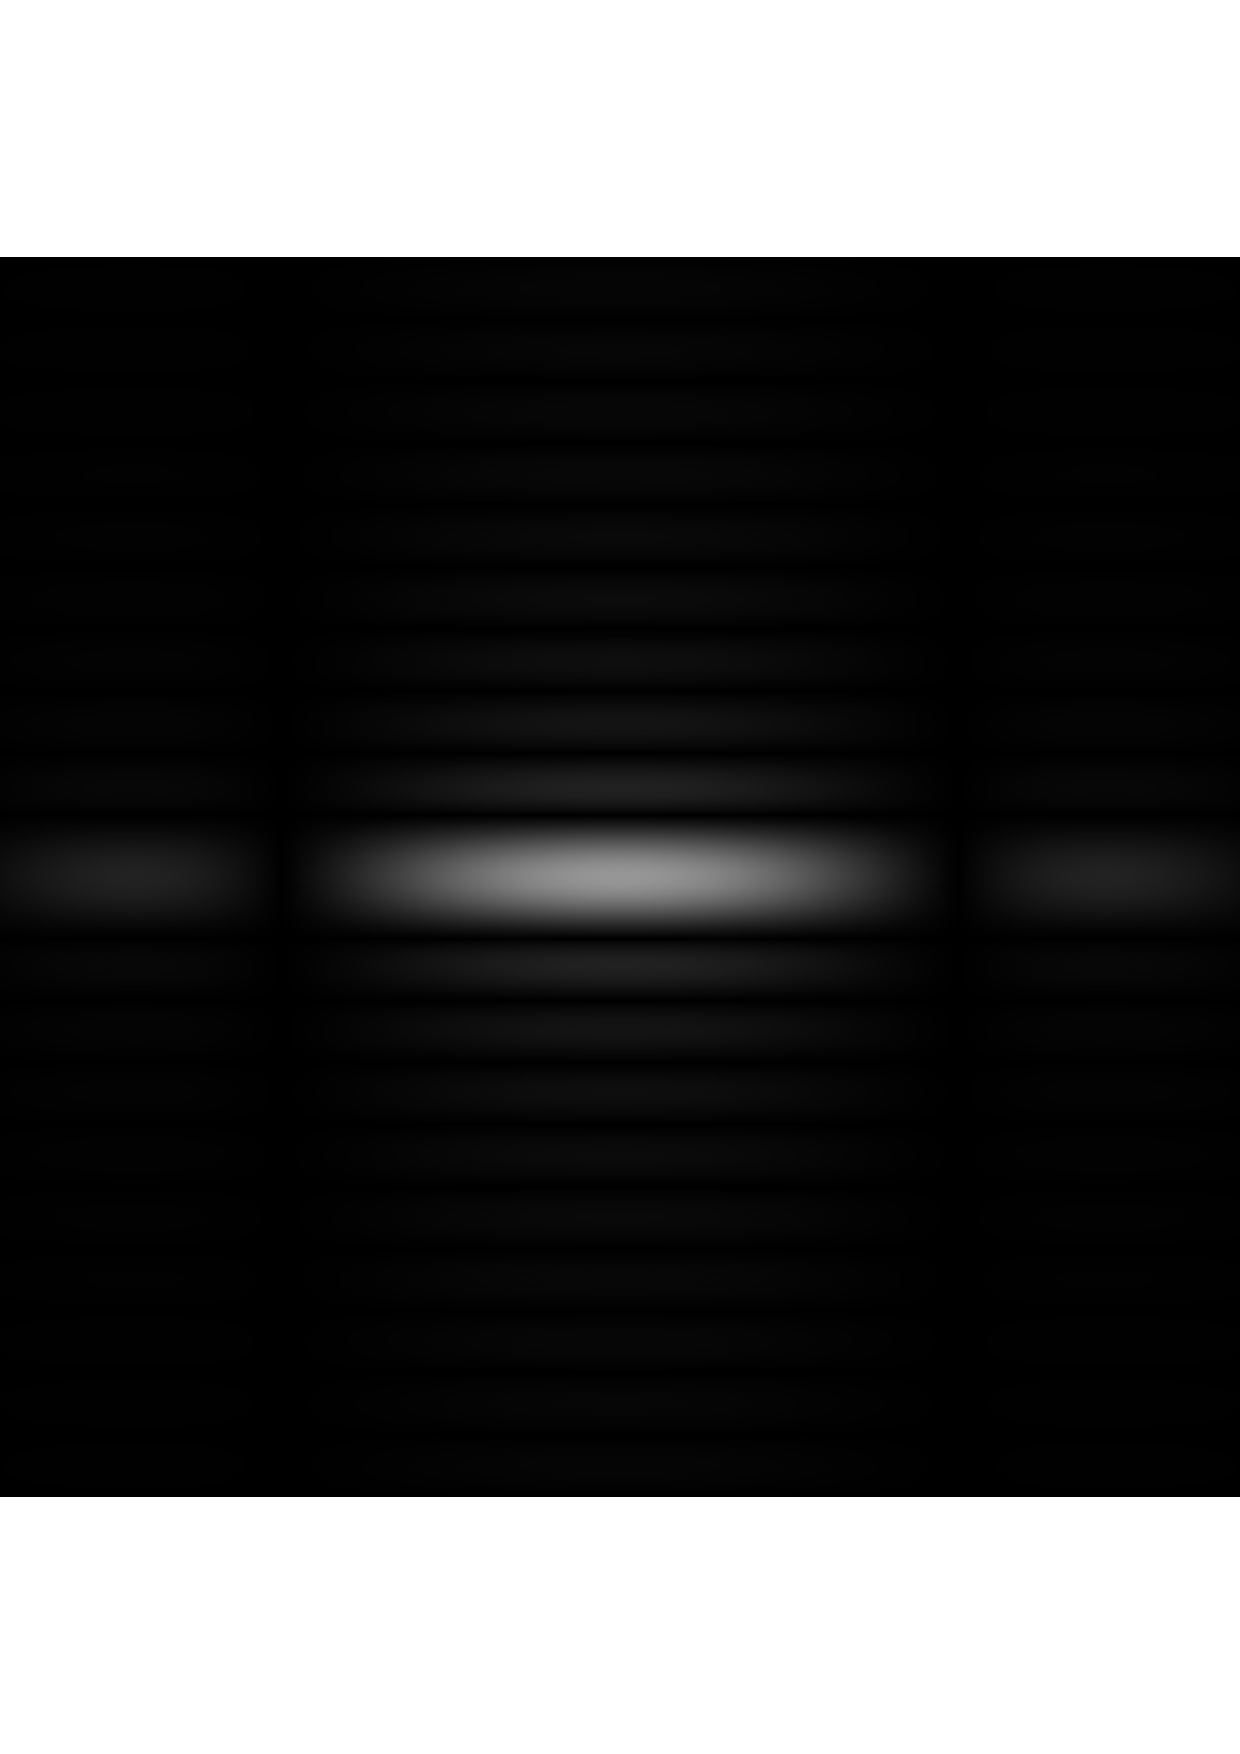
\includegraphics[width=0.20\textwidth]{img/2_1.bmp.pdf}
     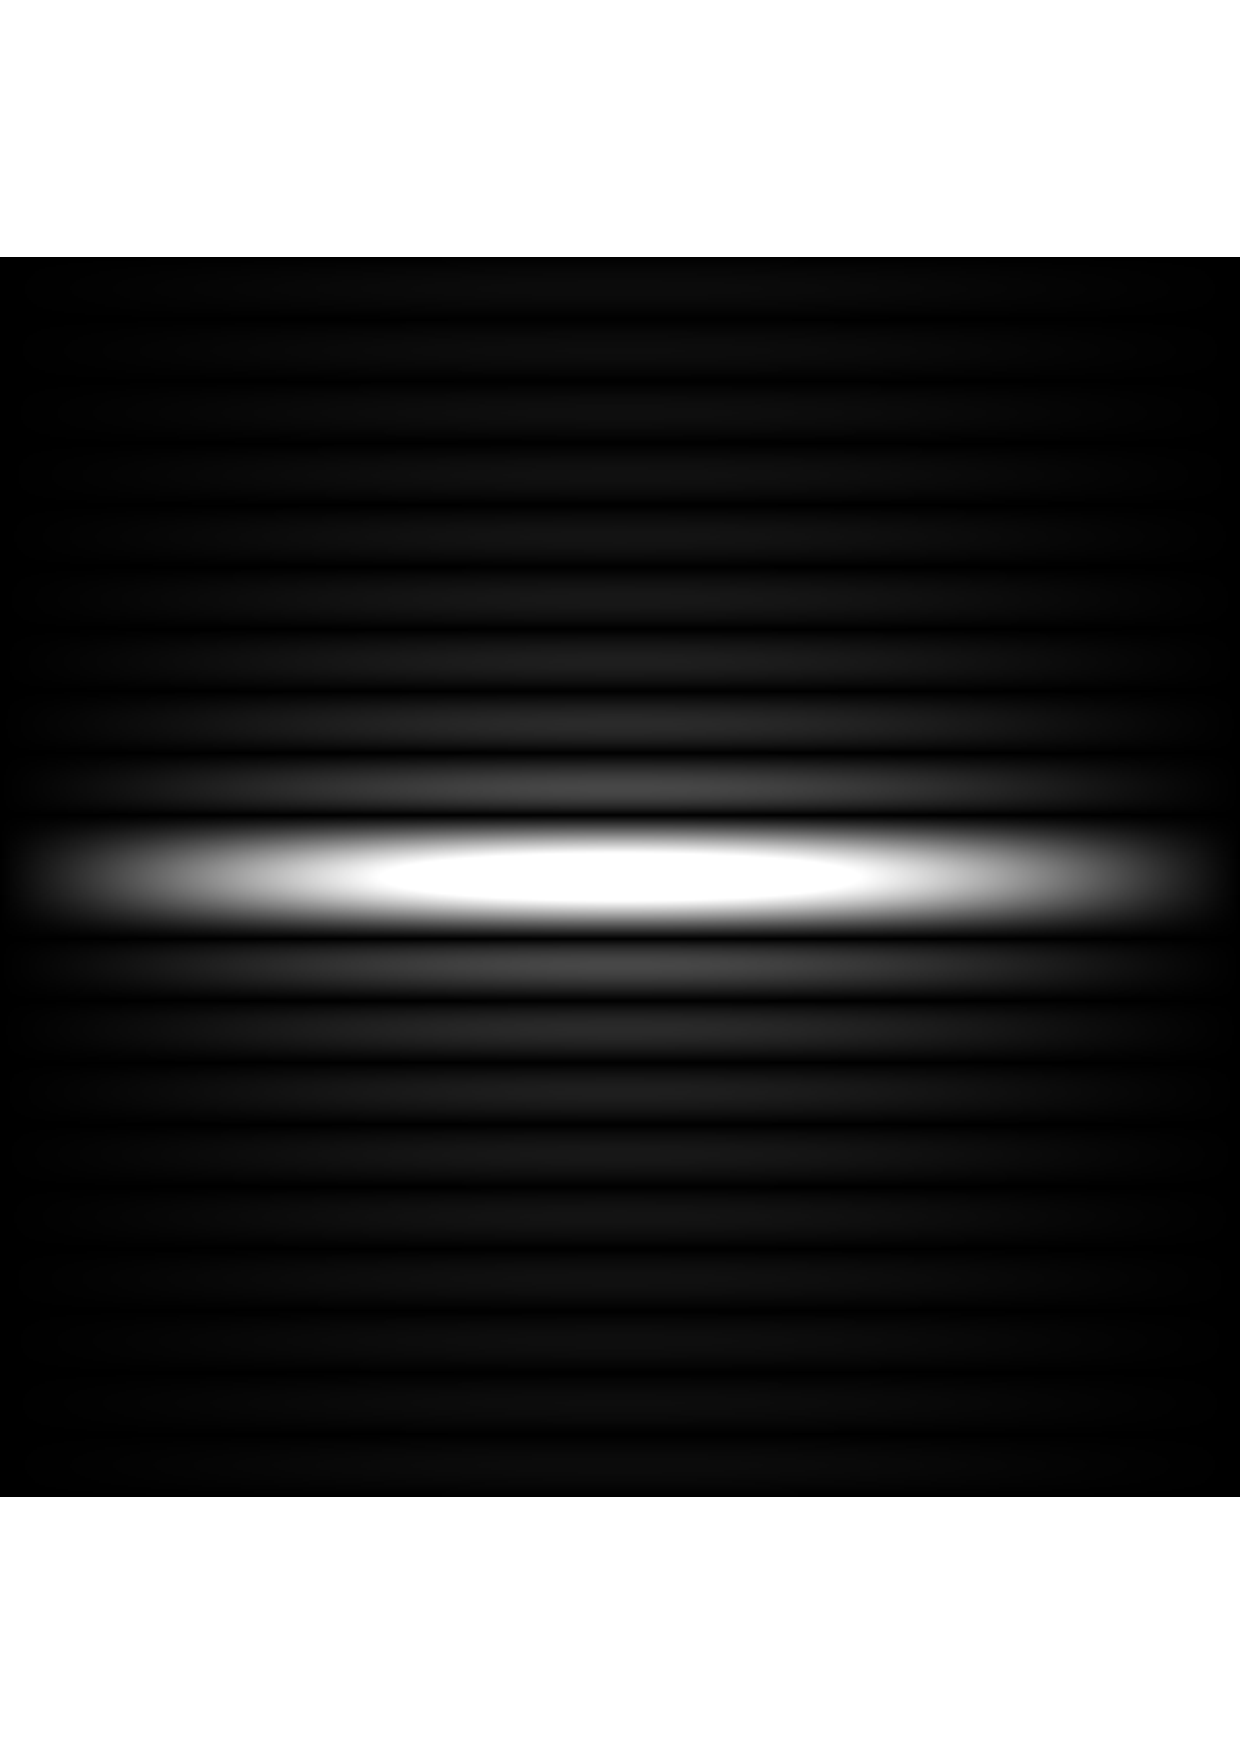
\includegraphics[width=0.20\textwidth]{img/2_2.bmp.pdf}
     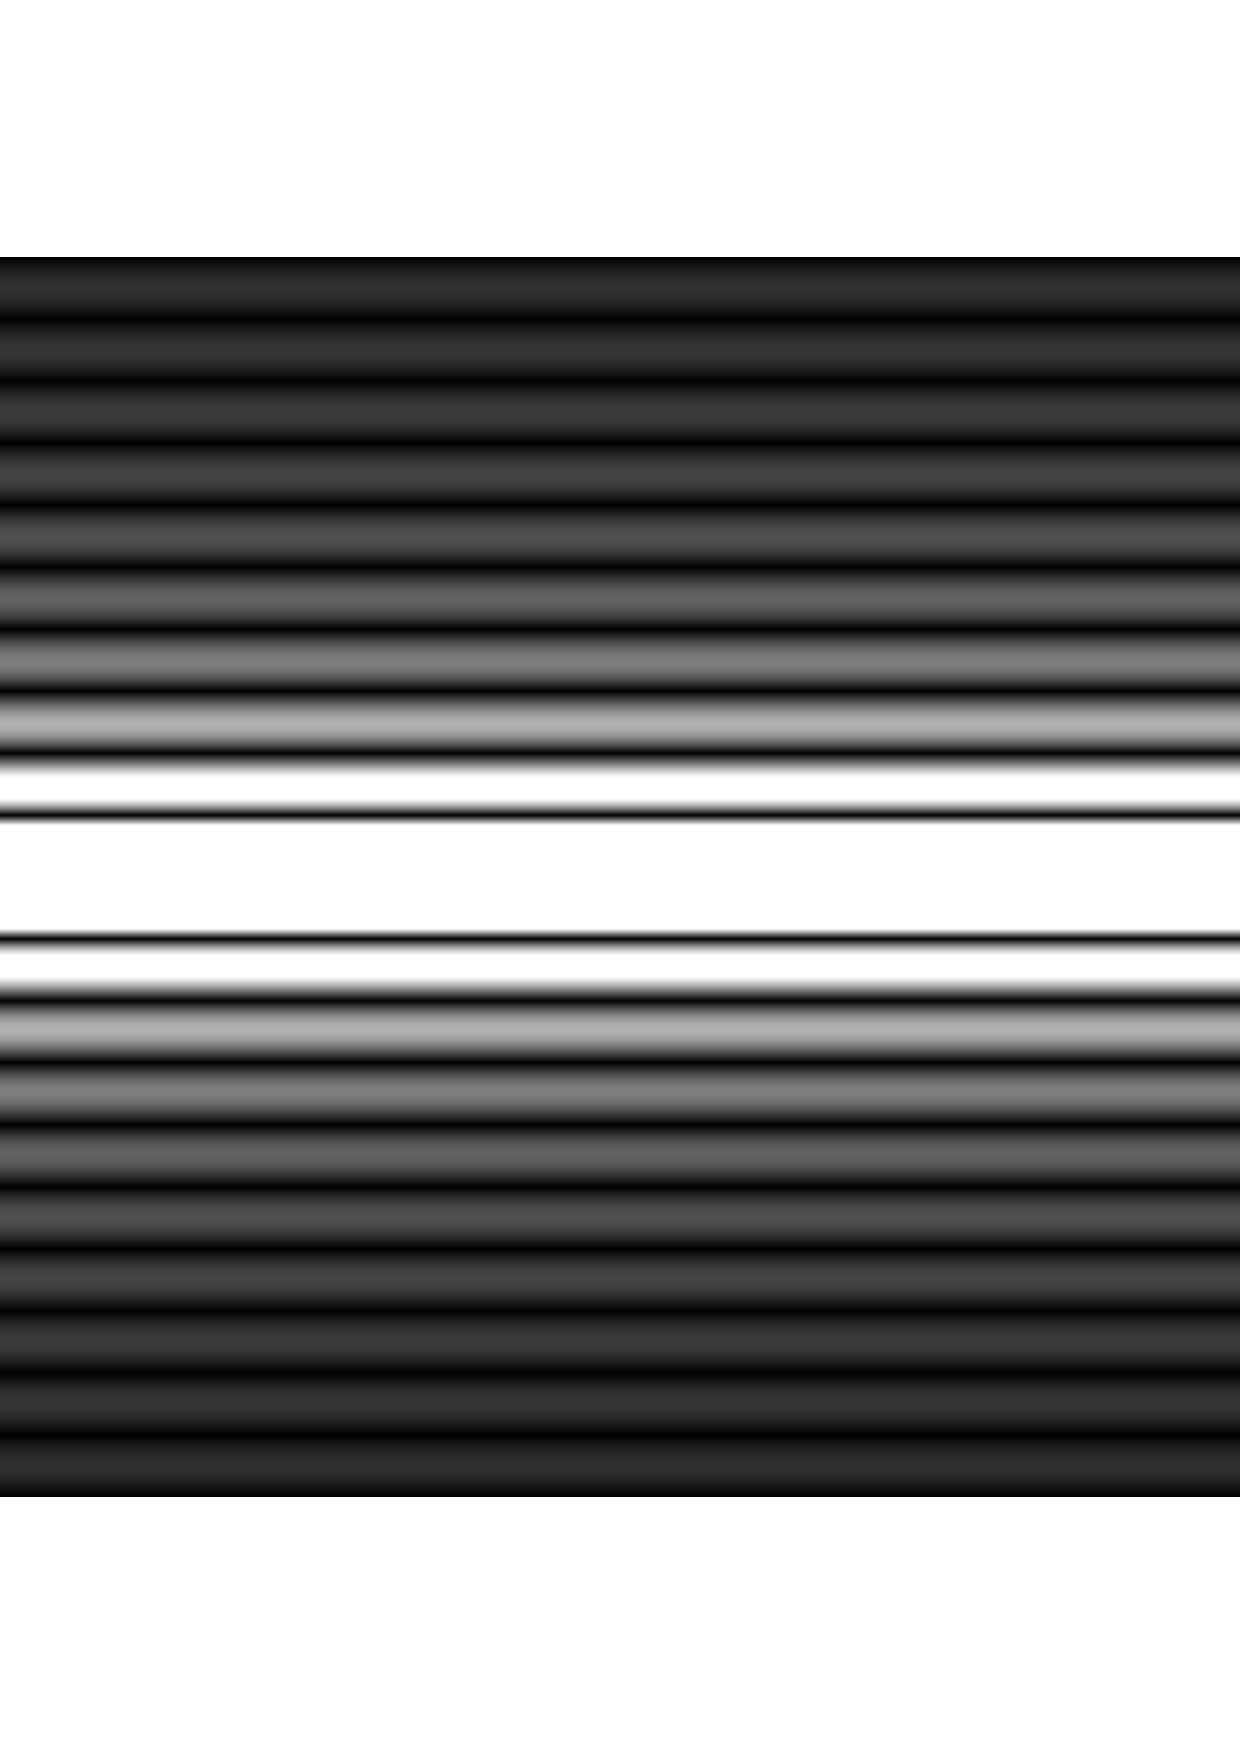
\includegraphics[width=0.20\textwidth]{img/2_3.bmp.pdf}
     \caption{Fraunhofer diffraction patterns as height at $0.0001m, 0.0005m, 0.001m$ and $0.005m$.}
     \label{fig2.1}
\end{figure}

%=================================================================================================
\pagebreak
%=================================================================================================
%TASK 3
%-------------------------------------------------------------------------------------------------
\section{\uline{TASK 3}}
%-------------------------------------------------------------------------------------------------
The beamwidth function $w(z)$ can be written as
\begin{equation}
    w(z)=\sigma \sqrt{1+\left(\frac{z}{z_{\mathrm{R}}}\right)^{2}}
    \label{w}
\end{equation}
with $z_{\mathrm{R}}=\frac{\pi \sigma ^{2}}{\lambda}$.

Apply $\sigma _1 = 3.9 \times 10^{-7}m$ and $\sigma _2 = 3.63 \times 10^{-6}m$ 
into function \ref{w}, we can draw the plot as below.
\begin{figure}[H]
    \centering
     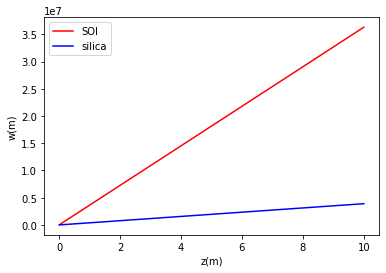
\includegraphics[width=0.6\textwidth]{img/task3_plot.png}
     \caption{The beamwidth function of SOI and silica}
     \label{fig3.1}
\end{figure}
%=================================================================================================
\pagebreak
%=================================================================================================
%TASK 4
%-------------------------------------------------------------------------------------------------
\section{\uline{TASK 4}}
%-------------------------------------------------------------------------------------------------
Opening circular aperture is a low-pass filter, which can filter out 
the high frequency components and only allow the low frequency components through. 
As Fig\ref{fig4.1} shown, the high frequencies of the oscillation are filtered out, 
leaving only the low frequencies. In Fig\ref{fig4.2}, the 2D image also loses its original shape 
and became blurry around the edges. 
\begin{figure}[H]
    \centering
     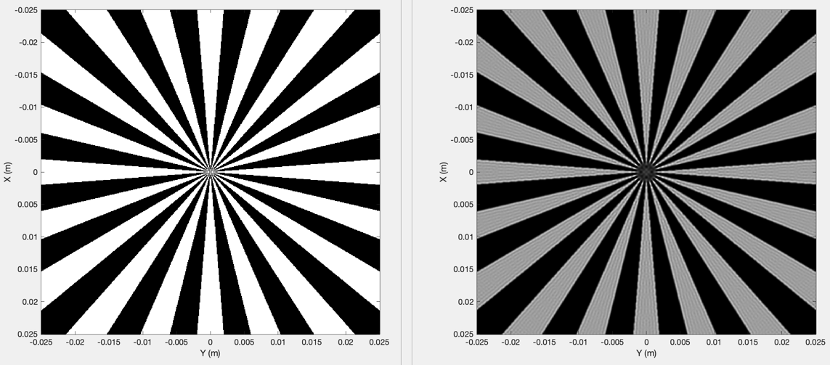
\includegraphics[width=0.8\textwidth]{img/7_1.png}
     \caption{Opening circular aperture graph(1d)}
     \label{fig4.1}
\end{figure}
\begin{figure}[H]
    \centering
     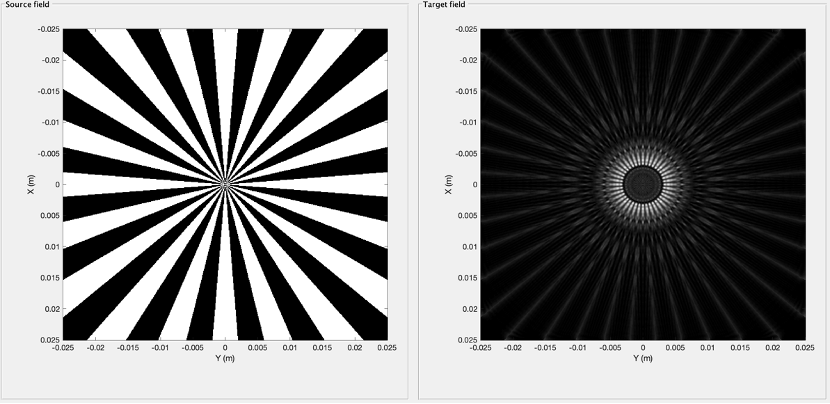
\includegraphics[width=0.8\textwidth]{img/7_2.png}
     \caption{Opening circular aperture graph(2d)}
     \label{fig4.2}
\end{figure}

Blocking one is a high-pass filter, which can filter out the low frequency components 
and only allow the high frequency components to pass through. 
It can be seen from Fig\ref{fig4.3} that the high frequency part of the oscillation is 
retained, while the low frequency part is filtered out. 
In Fig\ref{fig4.4}, the 2D image retains the edges of the original image, 
with Lena’s figure clearly visible and the smooth brightness changes disappearing.
\begin{figure}[H]
    \centering
     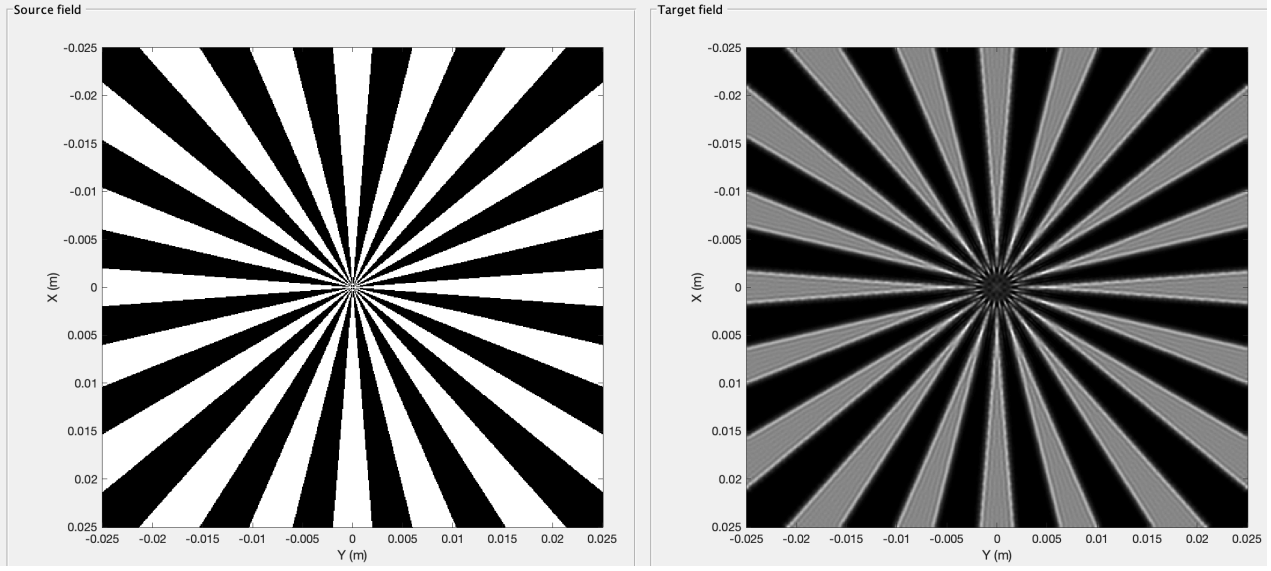
\includegraphics[width=0.8\textwidth]{img/7_3.png}
     \caption{Blocking circular aperture graph(1d)}
     \label{fig4.3}
\end{figure}
\begin{figure}[H]
    \centering
     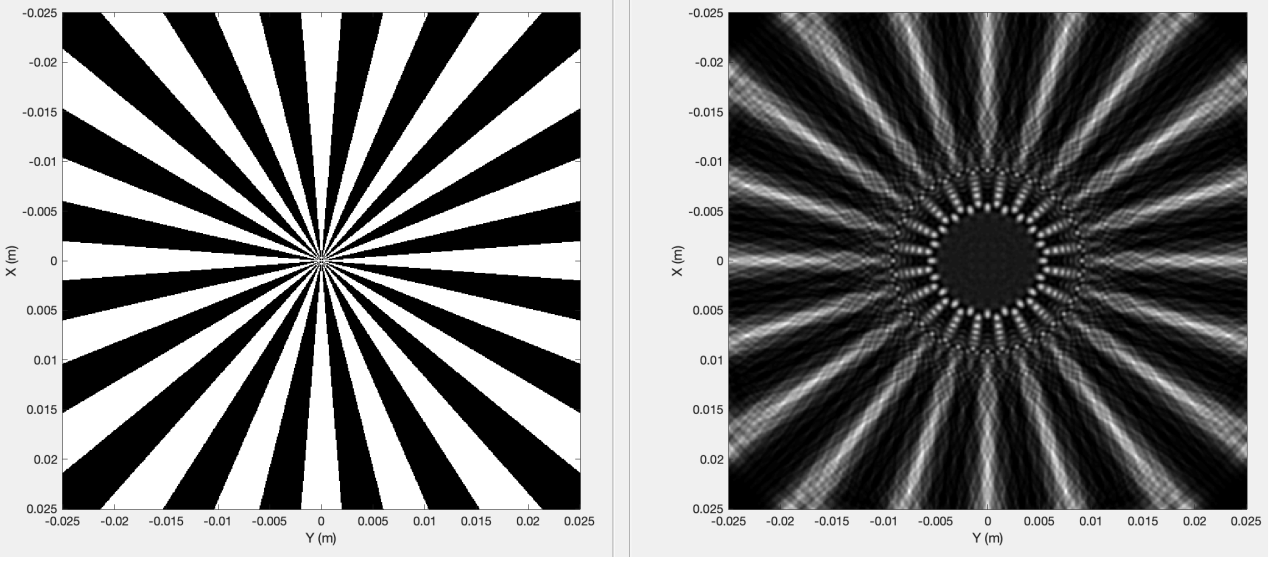
\includegraphics[width=0.8\textwidth]{img/7_4.png}
     \caption{Blocking circular aperture graph(2d)}
     \label{fig4.4}
\end{figure}
%=================================================================================================
\pagebreak
%=================================================================================================
%CTASK 5
%-------------------------------------------------------------------------------------------------

%=================================================================================================
%Appendix A
%-------------------------------------------------------------------------------------------------
% \section*{\uline{APPENDIX A}}
% %-------------------------------------------------------------------------------------------------
% Here comes some text. This text makes use of 1.5 line spacing. %=================================================================================================
% \pagebreak
%=================================================================================================
% %Appendix B
% %-------------------------------------------------------------------------------------------------
% \section*{\uline{APPENDIX B}}
% %-------------------------------------------------------------------------------------------------
% Here comes some text. This text makes use of 1.5 line spacing.\\
% In order to cite use \cite{Bern:1}, \cite{Bez:1}, \cite{BioModels}, \cite{Row:1} %=================================================================================================
% \pagebreak
% %=================================================================================================
% \bibliographystyle{plain}
% \bibliography{References}
%=================================================================================================

\end{document}